\section{The Body}
\label{sect:body}

Humans become skillful at controlling their own body after a long period of postnatal development and probably thousands of trials. Similarly the robot spends the first phase of its artificial development learning how to correctly control the head and the arm to perform various tasks such as visual tracking and reaching for a visually identified target.

Control of the body requires implicit knowledge of its structure (relative position of the limbs, their size, etc.) as well as its dynamical characteristics (e.g. the weight of the body segments). The ensemble of this knowledge is called \emph{body-schema}; experiments in neuroscience have given support to the existence of a body-schema in the primate brain \cite{graziano99whereis,graziano00coding}. Graziano and co-workers have found neurons in the motor cortex of the monkey, which code the position of the hand in the visual field.

On the other hand, developmental psychologist have been trying to understand the mechanisms which allow the brain to acquire such a representation. As roboticists we are interested in the same mechanisms as they allow the system (biological or artificial) to autonomously acquire and maintain all parameters required to the control of action and avoid their manual estimation and calibration. For this reason the problem has been studied by many authors \cite{yoshikawa03doestheinvariance,fitzpatrick04feelthebeat,metta03early}.

We follow here an approach similar to the one of \cite{fitzpatrick04feelthebeat,metta03early} where repeated self-generated actions are exploited for learning. We programmed the robot to perform a periodic movement of the wrist. This motion is observed by the robot visually and \emph{motorically}. In the former case the visual motion is computed by image differencing with an adaptive model of the background. In the latter case the robot computes the first derivative of the encoder feedback. The period of motion of each pixel in the motion image is compared to that of the encoder. Pixels whose motion is periodic and whose period matches that of the joints are selected and grouped together to form the segmentation of the hand. Figure \ref{fig-handsegmentation} shows an example of the result of this procedure.

\begin{figure}
\centering
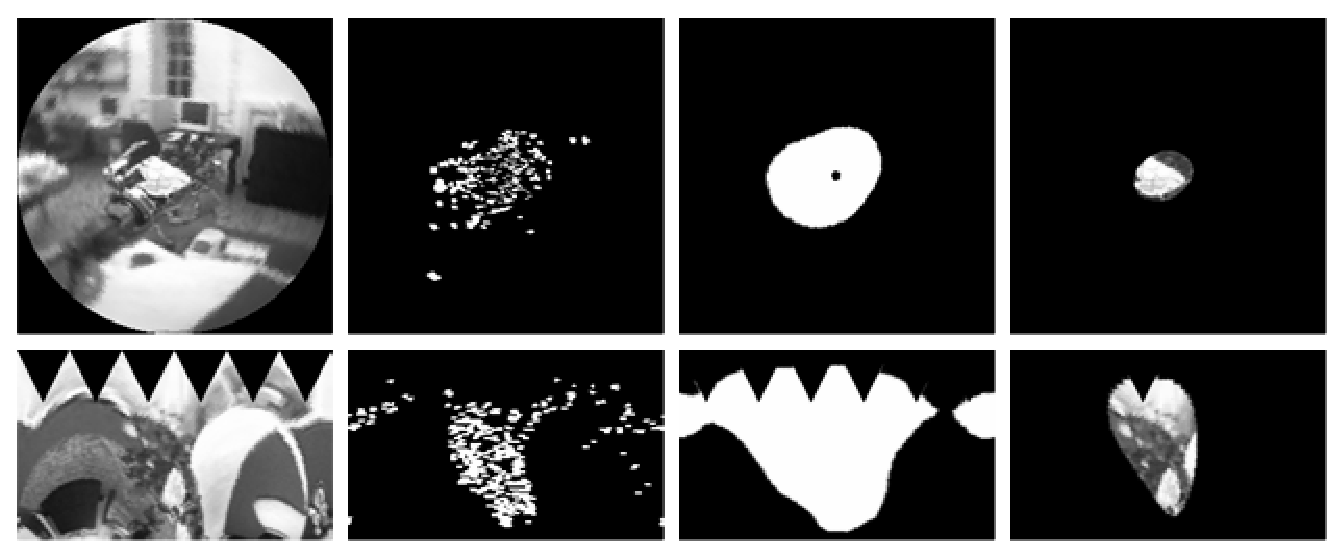
\includegraphics[width=3in]{handsegmentation}
\caption{Hand segmentation: an example.}
\label{fig-handsegmentation}
\end{figure}

We used this procedure to train a neural network to estimate the position of the hand in the visual field given the current robot posture (arm and head joint configuration). Another neural network learns the approximate shape and orientation of the hand given the same segmentation information. Figure ~\ref{sec-handlearning1} show the result of this procedure. 

The role of vision during reaching is still debated \cite{saunders03humans}, although experimental results suggest that the sight of the hand is not required for children to start reaching for an object \cite{clifton93isvisually,clifton94multimodal} and it is used only relatively late in development to actually adjust the trajectory of the hand during action \cite{ashmead93visual}. 

Sight of the hand, however, might be used to acquire eye-hand coordination. By tracking the hand the robot builds a mapping between the position of the arm and the corresponding head configuration when fixation is achieved. The hypotheses is that reaching starts by first fixating the object; in this condition the fixation point coincides with the target and uniquely identifies its position with respect to the body. The arm motor command can be obtained by a transformation between the head and arm joint angles, that is by mapping motor variables into motor variables:
\begin{equation}q_{arm}=f(q_{head})\label{motormapping}\end{equation}
\noindent where $q_{arm}$ and $q_{head}$ are head and arm posture respectively. This mapping implicitly implements the inverse kinematics of the arm and it can be learned when the robot looks at its hand: that is, the robot can maintain the fixation of the hand while moving the arm randomly in the workspace. Every time the arm stops and the eyes have achieved a stable fixation of the hand, a new pair of arm-head positions is acquired and used as a training sample to the neural network approximating the mapping of equation \ref{motormapping}. The robot uses the mapping to reach for visually identified objects as soon as a few samples are acquired.

The actual trajectory is computed by linearly interpolating the motor command and the current joint position. The trajectory results in a set of small changes that are effected by a PD controller with gravity compensation. A procedure to learn the gravity component is explained in \cite{natale04thesis}.

\begin{figure}
\centering
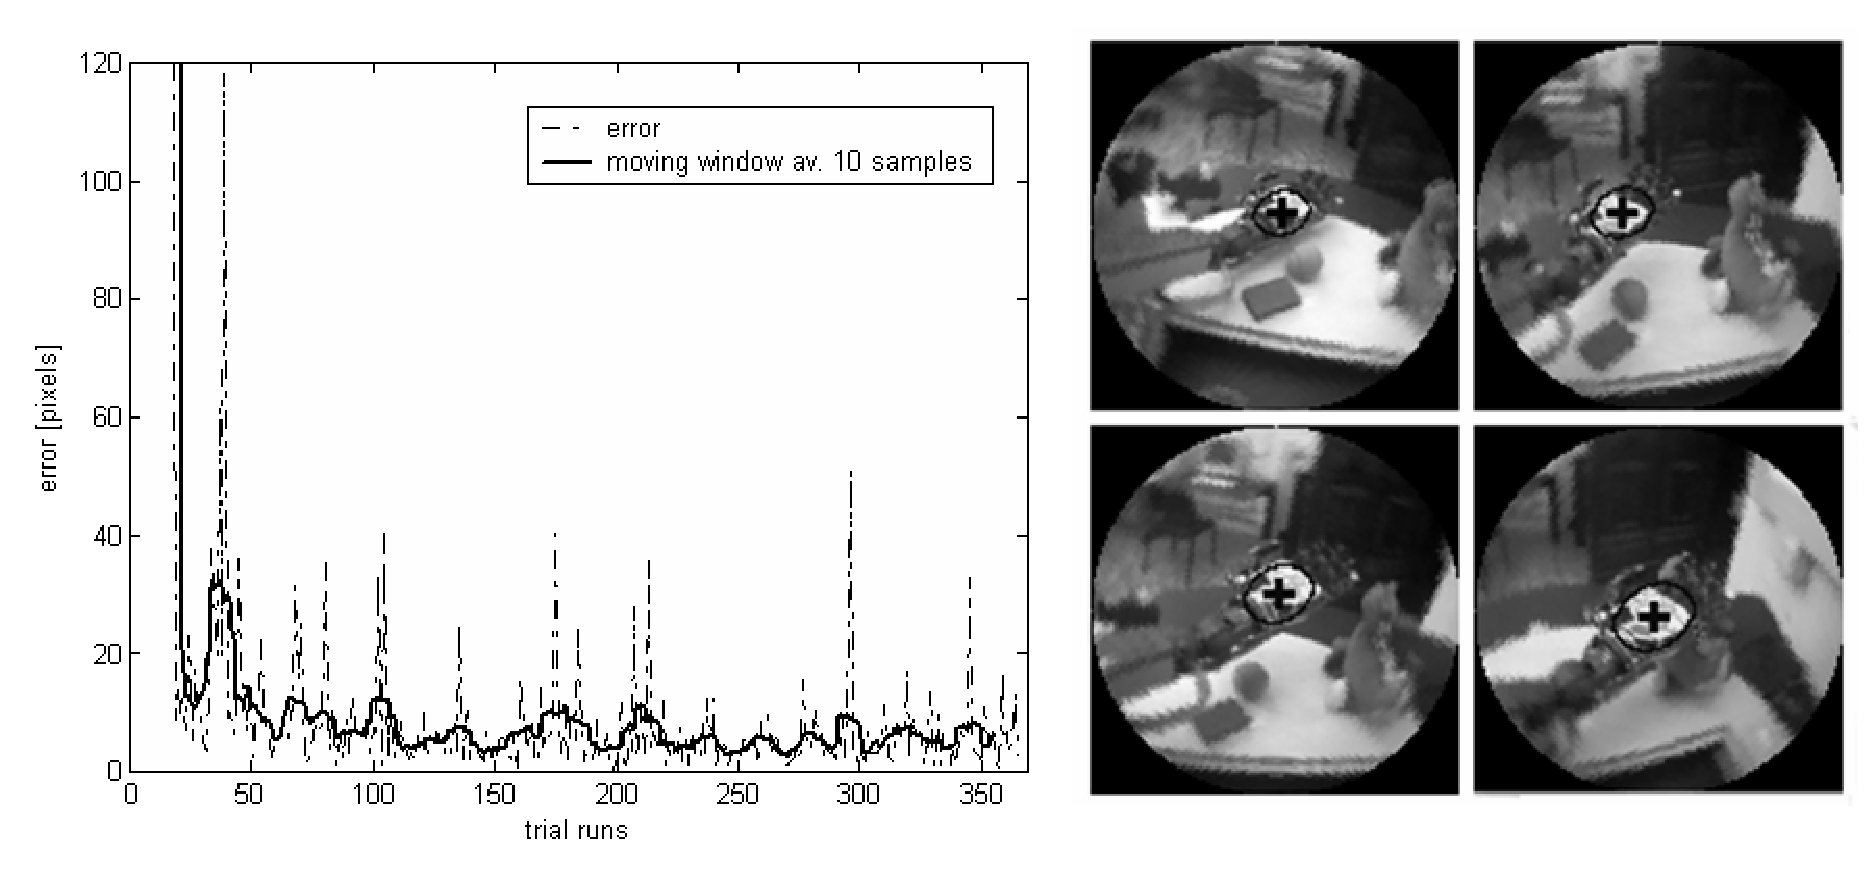
\includegraphics[width=3.5in]{handlearning1}
\caption{Learning to localize the hand in the visual field. The convergence of the approximation error as result of training of the neural network (left) and a few exemplar frames of the subsequent prediction (right).}
\label{sec-handlearning1}
\end{figure}

